

\tikzset{every picture/.style={line width=0.75pt}} %set default line width to 0.75pt        

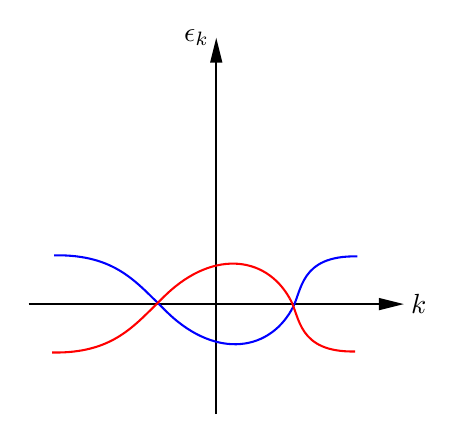
\begin{tikzpicture}[x=0.75pt,y=0.75pt,yscale=-1,xscale=1]
%uncomment if require: \path (0,300); %set diagram left start at 0, and has height of 300

%Straight Lines [id:da8505610866933] 
\draw    (101,219) -- (279.71,219) ;
\draw [shift={(281.71,219)}, rotate = 180] [fill={rgb, 255:red, 0; green, 0; blue, 0 }  ][line width=0.08]  [draw opacity=0] (12,-3) -- (0,0) -- (12,3) -- cycle    ;
%Straight Lines [id:da8248225909624645] 
\draw    (191.35,272) -- (191.35,92.69) ;
\draw [shift={(191.35,90.69)}, rotate = 450] [fill={rgb, 255:red, 0; green, 0; blue, 0 }  ][line width=0.08]  [draw opacity=0] (12,-3) -- (0,0) -- (12,3) -- cycle    ;
%Curve Lines [id:da9081456724098811] 
\draw [color={rgb, 255:red, 0; green, 0; blue, 255 }  ,draw opacity=1 ]   (166.29,221.5) .. controls (189.07,244.89) and (215.79,243) .. (227.79,221.5) ;
%Curve Lines [id:da5382231783747533] 
\draw [color={rgb, 255:red, 0; green, 0; blue, 255 }  ,draw opacity=1 ]   (113.29,195.5) .. controls (142.79,195) and (152.79,208.5) .. (166.29,221.5) ;
%Curve Lines [id:da8190264329883021] 
\draw [color={rgb, 255:red, 0; green, 0; blue, 255 }  ,draw opacity=1 ]   (259.29,196) .. controls (231.29,195.5) and (232.79,213) .. (227.79,221.5) ;

%Curve Lines [id:da487854281259237] 
\draw [color={rgb, 255:red, 255; green, 0; blue, 0 }  ,draw opacity=1 ]   (165.29,216.33) .. controls (188.07,192.94) and (214.79,194.83) .. (226.79,216.33) ;
%Curve Lines [id:da8067779262113395] 
\draw [color={rgb, 255:red, 255; green, 0; blue, 0 }  ,draw opacity=1 ]   (112.29,242.33) .. controls (141.79,242.83) and (151.79,229.33) .. (165.29,216.33) ;
%Curve Lines [id:da43392835439828703] 
\draw [color={rgb, 255:red, 255; green, 0; blue, 0 }  ,draw opacity=1 ]   (258.29,241.83) .. controls (230.29,242.33) and (231.79,224.83) .. (226.79,216.33) ;


% Text Node
\draw (283.71,219) node [anchor=west] [inner sep=0.75pt]    {$\boldsymbol{k}$};
% Text Node
\draw (189.35,90.69) node [anchor=east] [inner sep=0.75pt]    {$\epsilon _{\boldsymbol{k}}$};


\end{tikzpicture}
